% figures/budget-conformance.tex — per-repo outline token-budget conformance.
% Data: data/aggregated/outline-budget.csv (col `within_budget_pct`).
% Budget B = 300 tokens (§6.3). Go-only Phase 1a corpus (n=200 per repo).
% Target line at 95% marks the paper's §6.3 success criterion.
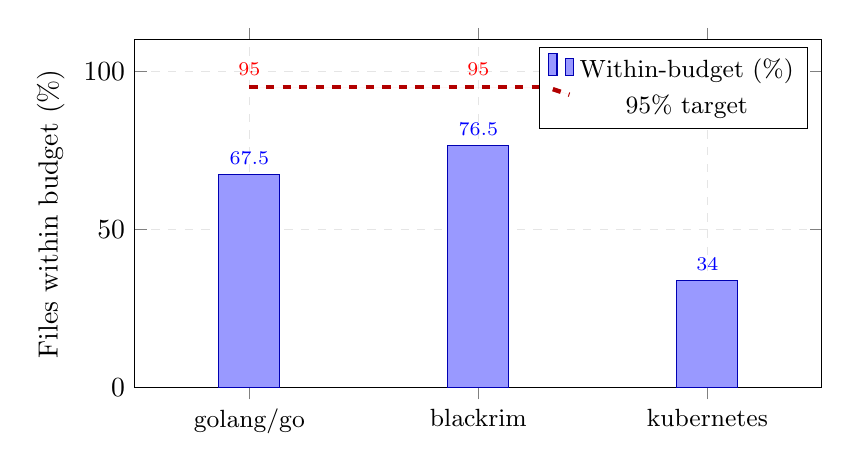
\begin{tikzpicture}
\begin{axis}[
    width=0.85\textwidth,
    height=6cm,
    ybar,
    bar width=22pt,
    ymin=0, ymax=110,
    enlarge x limits=0.25,
    ylabel={Files within budget (\%)},
    symbolic x coords={golang/go, blackrim, kubernetes},
    xtick=data,
    xticklabel style={font=\small},
    nodes near coords,
    nodes near coords align={vertical},
    nodes near coords style={font=\scriptsize, /pgf/number format/.cd, fixed, precision=1},
    grid=major,
    grid style={dashed,gray!20},
    legend style={at={(0.98,0.98)}, anchor=north east, font=\small},
]
% Measured within-budget percentages from data/aggregated/outline-budget.csv.
% Token estimate: Markdown output chars/4 (primary); B=300 tokens.
% Corpus: golang/go@release-branch.go1.22, kubernetes@release-1.30,
%         jsgerman-oss/blackrim.dev@HEAD. n=200 per repo, LoC≥200 filter.
\addplot+[fill=blue!40, draw=blue!70!black] coordinates {
  (golang/go,   67.5)
  (blackrim,    76.5)
  (kubernetes,  34.0)
};
% 95% target line from §6.3
\addplot+[
    sharp plot,
    no marks,
    ultra thick,
    draw=red!70!black,
    dashed,
] coordinates {
  (golang/go,  95)
  (blackrim,   95)
  (kubernetes, 95)
};
\legend{Within-budget (\%), 95\% target}
\end{axis}
\end{tikzpicture}
